\chapter{Recursos avançados}
A maior parte do básico está feito.  Você sabe escrever, sabe apagar, sabe
trocar palavras de lugar, copiando e colando.  Já aprendeu a pular dentro
de um arquivo, fazendo parecer bruxaria.  Mas até agora estamos no reino
iluminado, em que se um iniciante observar pode conseguir entender o que
está acontecendo.  Eu diria que a partir de agora vamos mexer com magia
negra, pois se faltar atenção, nada será absorvido.  Por isso, a partir
daqui, teste tudo e crie você mesmo experimentos.

Vamos começar falando sobre como procurar e substituir termos e palavras
chave num arquivo e como podemos substituir estes.  Na sequência veremos o
que são os registros e para onde vão os trechos que apagamos.

Na sequência começaremos a usar múltiplos arquivos e executar ações neles.
Iremos organizar janelas para obter uma boa visualização, além de montar e
manter um layout eficiente.

\section{Busca No Arquivo}
Buscar dentro do arquivo é relativamente simples.
Basta usar o comando \vimcommand{/} e pesquisar o que você deseja encontrar.
Se for encontrado o termo, seu cursor será jogado para cima dele.
Se você estiver usando o vim completo, ao habilitar a opção \vimcommand{:set hlsearch},
suas buscas serão destacadas do texto com uma cor de fundo diferente.
Para que o destaque desapareça, é preciso rodar um comando,
\vimcommand{:nohlsearch}, ou a versão reduzida \vimcommand{:noh}. 

Para avançar entre os termos encontrados na busca, use o comando \vimcommand{n} para avançar.
Para retroceder, buscando termos anteriores, use \vimcommand{N}.
Na régua inferior podem aparecer informações importantes do tipo, "Sua busca chegou ao fim do arquivo, recomeçando",
vale a pena ficar de olho.

\insertfigure{scale=0.70}{recursos_avancados/Busca_No_Arquivo.jpg}{Mecanismo de busca com HighlightSearch.}

Podemos realizar buscas no sentido inverso do arquivo com \vimcommand{?}, que terá os mesmos impactos que a busca normal.
Caso você queira buscar um termo que esteja sob o cursor, pode-se utilizar \vimcommand{\#},
que o mesmo efeito de se utilizar a busca com \vimcommand{/} ocorrerá. 
Para se buscar o termo sob o cursor, mas no sentido inverso, vale o comando \vimcommand{*}\ .

Se você realizou uma busca e deseja repetí-la, \vimcommand{//}, e o mesmo vale para \vimcommand{??}.

O mecanismo de busca funciona normalmente no vim tiny, mas sem esse destaque.
Isso pode tornar difícil realizar uma busca válida, já que você pode nãoperceber com antecedência
que está escrevendo errado no campo de busca.

\insertfigure{scale=0.70}{recursos_avancados/Busca_No_Arquivo_vimtiny.jpg}{No vimtiny temos a mesma potência, mas não a mesma elegância.}

Apesar de podermos pesquisar termos simples, podemos também utilizar expressões regulares para encontrar padrões que se casam com nossas especificações.
Este é um texto sobre vim, não sobre REGEX, então, se quiser, vá atrás por conta.

\section{Substituição No Arquivo}
Quando estamos programando temos o costume de usar vastamente palavras chave.
A repetição de palavras chave é muito grande, seja para nomear variáveis, seja para nomear funções,
ou mesmo uma informação escrita à força, ou \textit{hardcoded}.
Você pode realizar a substituição de diversas formas diferentes.
Como você já sabe realizar a busca, basta encontrar e substituir uma a uma.
Mas, se você deseja fazer de uma forma automática, que abrange de uma ocorrência, a múltiplas delas, então esse comando é pra você.

Para realizar a substituição de uma ocorrência, na linha atual, pode-se usar:\\
\vimcommand{:s/ocorr/subst}.

\begin{figure}
\begin{center}
	\fbox{
	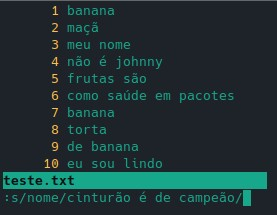
\includegraphics[scale=0.9]{recursos_avancados/Substituicao_simples.jpg}
	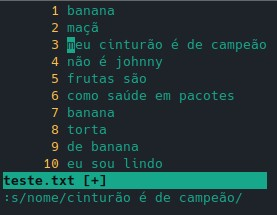
\includegraphics[scale=0.9]{recursos_avancados/Substituicao_simples_realizada.jpg}
	}
\caption{A substituição só ocorre na linha do cursor.}
\end{center}
\end{figure}

Perceba que você precisa estar com o cursor na linha alvo da substituição.
Se sua substituição tem como alvo todas as ocorrências de \textit{ocorr}, então,
com o cursor posicionado na linha alvo, \vimcommand{:s/ocorr/subst/g} dirá ao comando que
você deseja aplicar as substituições globalmente, alterando todas as ocorrências.

Para trabalhar com um escopo definido de linhas, existem duas formas: A primeira,
definir em quais linhas do arquivo a substituição ocorrerá.
Nesse formato fazemos \\
\vimcommand{:4,12s/ocorr/subst}
podendo aplicar na primeira ocorrência, ou em todas elas adicionando \vimcommand{g} ao final.
Neste exemplo, o escopo será da linha 4 à linha 12.

Uma outra forma de definir o escopo é selecionar com o modo visual o trecho
que sofrerá alteração.
Temos um pouco mais de flexibilidade neste caso, podendo selecionar pedaços de linha,
linhas inteiras,
blocos de texto\ldots\
E então, basta aplicar o comando.

Se quisermos que o escopo seja o arquivo inteiro, em todas as ocorrências, usamos \vimcommand{:\%s/ocorr/subst/g}.
O termo \% simboliza o próprio arquivo no vim.

\insertfigure{scale=1.20}{recursos_avancados/Substituicao_global.jpg}{A substituição global é muito poderosa, tome cuidado.}

\insertfigure{scale=1.20}{recursos_avancados/Substituicao_global_realizada.jpg}{Na barra inferior vemos quantas ocorrências foram afetadas.}

Para terminarmos sobre substuições, para que sejamos perguntados se queremos ou não substituir o termo de ocorrência:
\vimcommand{:\%s/ocorr/subst/gc}, o termo \vimcommand{c} adicionado é quem faz o serviço.

\section{Folds}
Existem casos em que você tem um parágrafo que deseja colapsar, ou seja, deixá-lo numa única linha para poder visualizar o restante.
Esta é mais uma funcionalidade que só existe no vim completo.
É útil para verificar a consistência do formato geral do texto, e para poder, por exemplo, verificar se todos os assuntos foram abrangidos.

Pessoalmente, acho raro utilizar, e difícil de configurar.
Mas caso você esbarre numa sequência de teclas estranhas, então melhor saber desfazer essas alterações.

A lista de teclas de ação são:
\begin{itemize}
    \item \vimcommand{zc} - Fechar uma dobra.
    \item \vimcommand{zo} - Abrir uma dobra.
    \item \vimcommand{zM} - Fechar todas as dobras.
    \item \vimcommand{zR} - Abrir todas as dobras.
    \item \vimcommand{za} - Abrir ou Fechar dobras.
\end{itemize}

Se você fechou uma dobra de texto, então poderá abrir.
Existem muitos métodos para identificar uma possível dobra que faça sentido.
Existem os métodos: \textit{indent}, \textit{diff}, \textit{syntax}, \textit{expr}, \textit{manual} e \textit{marker}.

Uma rápida explicação sobre o modo manual.
Utiliza-se \vimcommand{:set foldmethod=manual}, para ativar o método.
Seleciona-se uma quantidade de texto com o modo visual, e se usa o comando \vimcommand{:fold}.
Então você habilitou o trecho do texto a ser dobrável.
Eu considero uma forma trabalhosa, mas extremamente versátil.

\insertfigure{scale=0.70}{recursos_avancados/Fold_metodo_manual.jpg}{Folds são um assunto meio obscuro.}

\section{Registers}
Os registros do vim são os slots de memória de elementos salvos e deletados.
Nestes slots podem haver todos os tipos de informações.
Trata-se de conteúdo apagado, o clipboard do vim, nome do arquivo atual, do arquivo anteriormente aberto,
e macros, que são o conteúdo a seguir.

Para uma primeira experiência sobre os registros, vamos salvar um trecho de texto
em um slot específico: \vimcommand{''ax}, este comando irá ativar o registro \vimcommand{a}, e
o utilizará para armazenar o caractere que será apagado com o comando \vimcommand{x}.

Para colar um trecho de texto desse slot, o comando é parecido: \vimcommand{''aP}.
Perceba que escolhi utilizar o P maiúsculo, simplesmente para poder desfazer as alterações causadas pelo comando anterior.
Você pode visualizar quais registros estão sendo utilizados e seu conteúdo usando o comando \vimcommand{:registers}.
Se você vir caracteres esquisitos como \vimkeys{$<$80$>$} ou \vimkeys{\^}\vimkeys{M}, saiba que são caracteres especiais como 
enter, esc, ctrl-M, etc.
No meu vim em específico, como eu tenho algumas macros definidas, as ações de teclas especiais ficam salvas neste formato,
portanto, o vim possui um método próprio de armazenar caracteres de ação especiais.

\insertfigure{scale=0.75}{recursos_avancados/Registers.jpg}{Os registros armazenam todo tipo de informação.}

\section{Macros}
Macros fazem parte de um conjunto mágico de ferramentas que o vim possui.
Existem, para os editores de código, plugins para poder se aproveitar da movimentação que o vim oferece.
E de fato é muito bom poder se mover, saltar, salvar e fechar determinados arquivos.
Mas as macros são uma ferramenta muito específica, muito poderosa, que dificilmente pode ser imitada por um plugin.

Macros armazenam sequências de ações, sejam comandos, sejam inserção de texto, deleção ou substituição.
Literalmente qualquer coisa pode ser armazenada. Então, basta ativar a macro e sua ação será re-executada.

Vamos fazer um teste super simples.
A partir do modo normal pressione \vimcommand{q} e uma tecla para ser usada como registro.
No rodapé da janela você verá algo como \textit{''recording @a''}, que mostra que você está gravando
uma macro no registro "a".
Tecle novamente \vimcommand{q} para interromper a gravação.

Para testar, vamos fazer o seguinte:\vimcommand{qa0x\$xjq}.
Abrimos a gravação \vimcommand{q}, atribuímos o registro \vimcommand{a},
pedimos que retorne para o começo da linha \vimcommand{0}, que delete um caractere
\vimcommand{x}, que então pule para o fim da linha \vimcommand{\$}
e delete um caractere novamente \vimcommand{x}, e então descemos uma linha \vimcommand{j},
para enfim, encerrarmos a gravação \vimcommand{q}.

Difícil acompanhar apenas lendo, mas super simples de executar.
E talvez o mais importante, simples de replicar.
Para repetir esse conjunto de ações, selecione o número de repetições e use \vimcommand{$@$a}.
Essa macro deleta o primeiro e último caractere de uma linha e então pula para a linha seguinte.
Se você quisesse, por exemplo, deletar a primeira palavra de um conjunto de linhas, como faria?
Se a respostas for "à mão", então você está perdendo tempo e desperdiçando o potencial da ferramenta.

Para gravar macros, podemos utilizar dois tipos de operação.
Podemos sobrescrever um registro, que é o que fizemos no exemplo, mas podemos também adicionar novos comandos.
Basta pedir que seja gravada a macro num slot maiúsculo.
Ao usar \vimcommand{qAdiwjq}, estamos adicionando um "delete inner word" e um descer linha à macro salva no registro a.
Verifique com o comando \vimcommand{:registers} suas macros de teste.

Caso não tenha ficado claro, como as macros são armazenadas em um registro, podemos colá-las com \vimcommand{''aP}.
Isso será útil.
Caso pretenda alterar a macro, você pode colá-la, e alterá-la, e então voltar a salvar no slot.
Não é a maneira mais simples e elegante de se fazer isso, mas é uma forma.
O importante é perceber a complexidade e as aplicabilidades que macros possuem.

Quando falarmos de arquivos de configuração, o famoso vimrc, poderemos simplesmente colar nossa macro lá.
Dessa forma, teremos nossas macros sempre disponíveis, e poderemos criar macros cada vez mais elaboradas.
Pessoalmente possuo macros que servem de atalho para alguns comandos, outras para alteração de layout,
que é um tópico futuro, e uma com uma sequência de texto pré-definido.
O ponto negativo é gastar os slots, mas são muitos, e você pode simplesmente desativar essas configurações
futuramente, ou mesmo sobrescrever com um vazio.

\section{O Que É Um Buffer}
Quando programamos e precisamos reservar uma quantidade de memória do computador declaramos um buffer.
Basicamente, se trata de uma quantidade de memória reservada para operação.
Abrir arquivos é uma operação que requer um buffer, já que realizar alterações pequenas diretamente em arquivo
não é a melhor das ideias.
A estratégia é trazer para memória, alterar o trecho, e devolver as alterações para o armazenamento.

Quando você abre um arquivo, o vim cria um buffer.
Esse buffer representa seu arquivo.
Quando você salva, ele escreve as alterações no arquivo original.
E o mais importante, ninguém disse que não poderiam haver mais de um buffer.
Ou seja, vamos começar a abrir e editar mais de um arquivo por vez!

\section{Operando Com Múltiplos Arquivos}
Quando iniciamos o vim, podemos abrí-lo com um arquivo, como em \vimcommand{\$vim arquivo01.txt}.
Mas nada nos impede de abrir múltiplos, como em \vimcommand{\$vim arquivo01.txt arquivo02.txt}.
Quando abrimos dessa forma, imediatamente nos deparamos com o arquivo01.txt, mostrado em tela cheia,
sem indicações de que de fato abrimos o tal arquivo02.txt.
Para listar a pilha do buffer, usamos o comando \vimcommand{:ls}.
Perceba que eu disse pilha do buffer, e não lista de arquivos.
Não necessariamente iremos abrir arquivos, logo logo abriremos uma instância de terminal, e uma janela de navegação.

\insertfigure{scale=0.95}{recursos_avancados/Badd_ls.jpg}{Podemos carregar diferentes arquivos ao mesmo tempo.}

Para adicionar um novo buffer, mesmo que vazio, basta escrever \newline
\vimcommand{:badd nome\_do\_arquivo}.
Também temos o formato \vimcommand{:edit nome\_do\_arquivo}.
Não é muito clara a diferença entre eles, então fica a seu critério consultar o manual: \vimcommand{:help edit} e \vimcommand{:help badd}.
E para deletar temos duas formas: A primeira é escrever \vimcommand{:bdelete nome\_do\_arquivo}, mas
é uma forma problemática, já que requer lembrar o nome do arquivo.
Eu recomendo utilizar \vimcommand{:ls} e em seguida, pela numeração do buffer escolher qual será deletado:
\vimcommand{:bd 3} por exemplo.

Para saber o significado de cada um dos símbolos que acompanham a numeração dos buffers, veja o manual.
Também haverá uma explicação sobre o manual mais ao final do documento.

Antes de podermos transitar, saiba que, por padrão, o vim não te deixa sair de um buffer com modificações feitas.
Ele pede que você salve as alterações.
Por enquanto, para poder transitar sem necessidade de salvar, utilize o comando \vimcommand{:set hidden} para
que seja ignorado o estado do arquivo.
Futuramente iremos adicionar esse comando em nosso arquivo de configuração.
\begin{figure}
\begin{center}
	\fbox{
	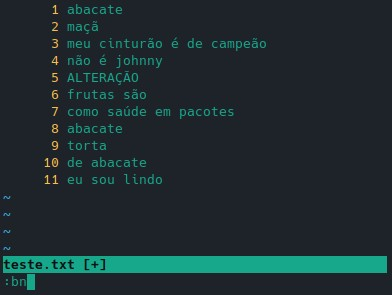
\includegraphics[height=5.4cm]{recursos_avancados/bn_setHidden.jpg}
	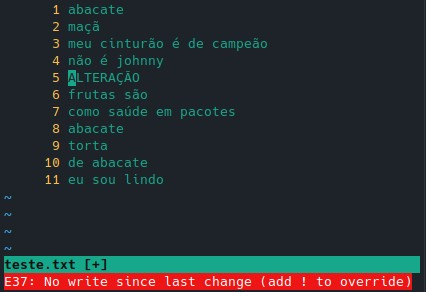
\includegraphics[height=5.4cm]{recursos_avancados/bn_error.jpg}
	}
\caption{Erro por não haver habilitado o modo hidden.}
\end{center}
\end{figure}

Agora que podemos adicionar e remover, vamos transitar entre os buffers, afinal de contas, é isso que interessa.
\vimcommand{:bnext} irá mudar para o próximo buffer da pilha.
\vimcommand{:bprevious} irá mudar para o buffer anterior da pilha.
\vimcommand{:bfirst} irá mudar para o primeiro buffer da pilha.
\vimcommand{:blast} irá mudar para o último buffer da pilha.
E pra finalizar, para pular para um buffer de número qualquer \vimcommand{:buffer \#}.

Todos esses comandos possuem formas simplificadas, exceto badd:
\begin{multicols}{2}
\begin{itemize}
    \item \vimcommand{:e} - Adicionar um buffer à pilha;
    \item \vimcommand{:badd} - Adicionar um buffer à pilha;
    \item \vimcommand{:bd} - Deletar um buffer da pilha;
    \item \vimcommand{:bn} - Ir ao próximo buffer;
    \item \vimcommand{:bp} - Ir ao buffer anterior;
    \item \vimcommand{:bf} - Ir ao primeiro buffer;
    \item \vimcommand{:bl} - Ir ao último buffer;
    \item \vimcommand{:b \#} - Ir ao buffer número \#;
\end{itemize}
\end{multicols}

Para abrir arquivos que estão inseridos dentro de pastas, ou que estão em pastas superiores,
depende-se de sintaxe de shell para caminhos relativos e absolutos, que eu suponho que você saiba.
Atenção, se você tentar abrir uma pasta acabará abrindo o navegador sem querer.
Teremos explicações sobre ele futuramente.

Existe um comando que abre todos os buffers numa janela, e isso entra no tópico a seguir.
Portanto, vou deixar aqui citado, e a explicação sobre como manipular fica no capítulo seguinte.
Para abrir todos os buffers na janela de uma só vez: \vimcommand{:ball}.

\insertfigure{scale=0.80}{recursos_avancados/ball_ls.jpg}{Vários buffers carregados.}

\vspace{1cm}
Apenas para citação: Existe um comando chamado bufdo, que executará uma ação em todos os buffers.
Com ele é possível rodar comandos, substituições e afins.
No entanto, a sintaxe é complexa, então vou deixar a cargo do leitor ir atrás de descobrir
se essas funcionalidades o são úteis.

\insertfigure{scale=0.80}{recursos_avancados/ball.jpg}{Usando \vimcommand{:ball} para abrir todos os buffers na janela.}

\section{MultiWindows}
Por hora conseguimos editar múltiplos arquivos.
A explicação sobre buffers serem como um espaço de memória, e sobre sua organização em pilhas
foi importante para sabermos como verificar quais arquivos estão carregados no vim.
Agora podemos dar passos significativos adiante.
Eu diria que esta é minha funcionalidade favorita desse editor.

Um detalhe importante que não citei antes por fazer diferença somente agora:
Existe uma diferença entre fechar com \vimcommand{:q} e deletar o buffer da pilha com \vimcommand{:bd}.
A diferença é que, com o comando \vimcommand{:q}, estamos fechando a janela em que o buffer se encontra,
mas se olharmos a lista de buffers com \vimcommand{:ls}, veremos que ele ainda está na pilha, e que,
portanto, pode ser novamente acessado.
Com \vimcommand{:bd} estamos descaregando da memória o arquivo, garantindo que as gravações foram ou feitas ou descartadas,
e liberando memória do editor.

\subsection{Invocando janelas}
Existem diversos comandos para abrir janelas.
Os dois primeiros, mais simples, são o \vimcommand{:new arquivo} que irá fazer com que a tela
se divida em duas horizontalmente, abrindo o novo buffer acima.
Já com o comando \vimcommand{:vertical new arquivo} o mesmo ocorre, mas verticalmente, e abrindo a nova janela à esquerda.

\insertfigure{scale=0.80}{recursos_avancados/split_new.jpg}{Abrindo uma nova janela.}

Outro conjunto, que faz mais jus ao nome das \textit{splitted Windows}, são os comandos \vimcommand{:split nome\_do\_arquivo} e 
\vimcommand{:vertical split nome\_do\_arquivo}.
Eles farão exatamente a mesma coisa que \vimcommand{:new} e \vimcommand{:vertical new}.

\insertfigure{scale=0.80}{recursos_avancados/vertical_split.jpg}{Abrindo uma janela vertical.}

Caso você já tenha carregado no editor a janela que deseja abrir, pode-se usar o comando
\vimcommand{:sbuffer}, ou \vimcommand{:vertical sbuffer}.
A vantagem de usar esse comando é a possibilidade de usar o comando \vimcommand{:ls}
para poder abrir a partir do número do buffer.

\insertfigure{scale=0.80}{recursos_avancados/vsbuffer.jpg}{Abrindo um buffer já carregado com vsbuffer.}
\insertfigure{scale=0.80}{recursos_avancados/vsbuffer_open.jpg}{Resultados semelhantes.}

Ficar limitado a sempre abrir à esquerda ou acima é complicado,
Mas temos a possibilidade de alterar qual será o local onde a nova janela irá nascer.

Como existem comandos para abrir verticalmente e horizontalmente, os comandos que definem
se a janela irá surgir acima/abaixo, na direita/esquerda, são colapsados.
E para complicar ainda mais, podemos por exemplo abrir logo à direita da janela atual, ou
abrir na extrema direita da tela.
E o mesmo para especificação vertical.

Para abrir algo logo abaixo ou à direita, use o comando \vimcommand{belowright}.
Perceba que, se usarmos o \vimcommand{split}, então ele irá mandar para baixo por conta do \vimcommand{below}.
Se usarmos o \vimcommand{vsplit}, irá abrir à direita, por conta do \vimcommand{right}.
Temos também os comandos \vimcommand{aboveleft},\vimcommand{botright}, e \vimcommand{topleft};
Com isso temos 8 combinações:
\vspace{1cm}

\begin{itemize}
    \item \vimcommand{:topleft split} - Abrir no topo da tela horizontalmente;
    \item \vimcommand{:botright split} - Abrir na base da tela horizontalmente;
    \item \vimcommand{:topleft vsplit} - Abrir no extremo esquerdo da tela verticalmente;
    \item \vimcommand{:botright vsplit} - Abrir no extremo direito da tela verticalmente;
    \item \vimcommand{:aboveleft split} - Abrir imediatamente acima da janela horizontalmente;
    \item \vimcommand{:belowright split} - Abrir imediatamente abaixo da janela horizontalmente;
    \item \vimcommand{:aboveleft vsplit} - Abrir imediatamente à esquerda da janela verticalmente;
    \item \vimcommand{:belowright vsplit} - Abrir imediatamente à direita da janela verticalmente;
\end{itemize}

\insertfigure{scale=0.80}{recursos_avancados/belowright_split.jpg}{Abrindo um buffer abaixo.}

Essas combinações realmente são muito ruins de se entender, principalmente por conta das indicações de direção
serem colapsadas em um único argumento.
Lembre-se, se o comando abre verticalmente, só importa esquerda e direita.
Se ele abre horizontalmente, só importa cima e baixo.

\insertfigure{scale=0.80}{recursos_avancados/aboveleft_vertical_sbuffer.jpg}{Efeito de aboveleft vertical sbuffer 4.}

\subsection{Alternando Entre Janelas E Movendo}
A forma mais simples de se mover entre janelas é usando \vimcommand{CTRL w CTRL w}, ou só \vimcommand{CTRL w w}.
Eu prefiro a primeira forma por já estar com o dedo no lugar.
Só com esse comando já podemos alternar legal entre as janelas. 
A lógica desse comando é alternar na ordem natural da escrita, que é, do topo para baixo, e da esquerda para a direita.

Mas claro que não vamos ficar limitados a esses movimentos simples.
O comando \vimcommand{CTRL w} habilita a movimentação.
Dessa forma, para ir para a janela da esquerda, basta usar \vimcommand{CTRL w l} para ir para a janela da direita.
Usando os comandos de movimentação \textit{hjkl} você se move para onde quiser.
Assim combinamos conhecimentos prévios:
\begin{itemize}
    \item \vimcommand{CTRL w h} - Troca para a janela da esquerda;
    \item \vimcommand{CTRL w l} - Troca para a janela da direita;
    \item \vimcommand{CTRL w j} - Troca para a janela debaixo;
    \item \vimcommand{CTRL w k} - Troca para a janela acima;
    \item \vimcommand{CTRL w t} - Troca para a janela superior (top);
    \item \vimcommand{CTRL w b} - Troca para a janela inferior (bottom);
\end{itemize}

\subsection{Redimensionando E Criando Um Layout}
Caso tenhamos aberto nossas janelas em uma disposição não muito agradável,
temos a opção de mover a janela para um dos cantos da tela.
Não temos como mover a janela com um controle muito bom, mas é melhor que nada.
Para mover a janela atual temos:

\begin{itemize}
    \item \vimcommand{CTRL w H} - Envia a janela atual para o canto esquerdo da tela;
    \item \vimcommand{CTRL w L} - Envia a janela atual para o canto direito da tela;
    \item \vimcommand{CTRL w J} - Envia a janela atual para o canto inferior da tela;
    \item \vimcommand{CTRL w K} - Envia a janela atual para o canto superior da tela;
    \item \vimcommand{CTRL w x} - Troca a janela atual de posição com seu vizinho mais próximo;
\end{itemize}

Podemos, por fim, redimensionar nossas janelas, seja com comandos, seja com atalhos.
Com comandos temos:

\begin{itemize}
    \item \vimcommand{CTRL w -} - Diminui verticalmente o tamanho da janela atual;
    \item \vimcommand{CTRL w +} - Aumenta verticalmente o tamanho da janela atual;
    \item \vimcommand{CTRL w $<$} - Diminui horizontalmente o tamanho da janela atual;
    \item \vimcommand{CTRL w $>$} - Aumenta horizontalmente o tamanho da janela atual;
    \item \vimcommand{CTRL w $|$ } - Aumenta verticalmente a janela atual ao máximo possível;
    \item \vimcommand{CTRL w \_ } - Aumenta horizontalmente a janela atual ao máximo possível (underscore);
\end{itemize}

No caso de redimensionar as janelas, é muito mais fácil editar algum atalho mais simples para a tarefa.
Eu particularmente deixo isso configurado, mas é bom saber qual o padrão, e saber mexer mesmo que não
seja na \textbf{sua} configuração.
É muito mais fácil alterar tamanho pedindo para redimensionar várias linhas ou colunas de uma vez.
Com atalhos conseguimos apenas uma linha ou uma coluna, ou os tamanhos máximos.
Os comandos abaixo estão escritos com o número 1, mas poderiam ser 5, 15, 55, o que o for razoável pra você.

Os comandos para alterar o tamanho das janelas são:
\begin{itemize}
    \item \vimcommand{:resize +1} - Aumenta verticalmente o tamanho da janela atual;
    \item \vimcommand{:resize -1} - Diminui verticalmente o tamanho da janela atual;
    \item \vimcommand{:vertical resize +1} - Aumenta horizontalmente o tamanho da janela atual;
    \item \vimcommand{:vertical resize -1} - Diminui horizontalmente o tamanho da janela atual;
    \item \vimcommand{:resize 35} - Torna o tamanho horizontal da janela como 35 linhas;
    \item \vimcommand{:vertical resize 35} - Torna o tamanho vertical da janela como 35 colunas;
\end{itemize}

Lembre-se, tamanho vertical refere-se à quantidade de colunas. Tamanho normal refere-se à quantidade de linhas.
Acabamos de encerrar o que há pra se saber sobre layout de janelas.

\insertfigure{scale=0.80}{recursos_avancados/resize.jpg}{Você pode manipular as dimensões das janelas à vontade.}

\section{MultiTabs}
Para quem entendeu a natureza de um buffer, e como as janelas servem apenas para mostrar os buffers
de maneira mais flexível, vai entender imediatamente as tabs (abas).
Assim como janelas organizam uma visualização de buffers, tabs organizam uma visualização de janelas.

Para criar uma nova aba, digamos uma aba com uma cópia do buffer atual, usamos o comando \vimcommand{:tabnew \%}.
Caso você tenha uma quantidade de abas abertas, e tiver o mouse ativado, você pode navegar clicando.
Também pode navegar por comando como \vimcommand{:tabNext}.

Caso você tenha uma quantidade de arquivos que deseja abrir, cada um em uma aba, na inicialização do vim,
pode-se usar \vimcommand{\$ vim -p arquivo1.txt arquivo2.py arquivo3.cpp}

Resumindo os comandos temos:
\begin{itemize}
    \item \vimcommand{:tabNew} - Cria uma nova aba;
    \item \vimcommand{:tabClose} - Fecha a aba atual. Não é o mesmo que deletar o buffer;
    \item \vimcommand{:tabprevious} - Move para a aba anterior;
    \item \vimcommand{gT} - Move para a aba anterior;
    \item \vimcommand{:tabmove -1} - Move a aba atual mais à esquerda na ordem das abas;
    \item \vimcommand{:tabnext} - Move para a próxima aba;
    \item \vimcommand{gt} - Move para a próxima aba;
    \item \vimcommand{:tabmove +1} - Move a aba atual mais à direita na ordem das abas;
    \item \vimcommand{:tabfirst} - Move para primeira aba.
    \item \vimcommand{:tablast} - Move para a última aba.
\end{itemize}

\insertfigure{scale=0.80}{recursos_avancados/tabnew.jpg}{Abas organizam layouts.}

Para mais informações, leia o manual com \vimcommand{:h tabpage}.
Usar abas é interessante para mover-se rapidamente entre arquivos que você sabe que utilizará.
Utilizar atalhos com estes comandos é uma grande vantagem.
Vreremos como configurar no vimrc.

\section{Save View}
Existem sessions e views como tentativas de salvar as configurações e layouts atuais.
Pessoalmente, nunca consegui utilizar direito as views, então vou deixar o manual aqui para você procurar:
\vimcommand{:help mkview}.
Acabamos de esgotar as funcionalidades do vim.tiny.
De agora em diante iremos utilizar somente prints do vim instalado completo.

\section{Netrw}
Caso você use o vim em sua versão completa, existe um navegador de arquivos embutido.
Num sistema com interface gráfica você certamente tem a capacidade de abrir um
explorador de arquivos, para navegar entre as diversas pastas que você não organiza.
Pois bem. O vim também tem algo parecido.

\insertfigure{scale=0.80}{recursos_avancados/netrwInicial.jpg}{Navegador de arquivos.}

O navegador NETRW nasceu como um plugin, mas atualmente está integrado ao vim.
E ainda bem que está.
Existem diversas formas de abrir o editor.
Pode-se usar o comando no terminal \vimcommand{\$ vim [pasta]} ou 
mesmo \vimcommand{\$ vim .}, e você estará no navegador de arquivos.
Mas e se você estiver dentro do vim, com seus arquivos já abertos?

Você pode usar o comando \vimcommand{:Explore} para carregar no buffer o explorador.
No entanto, agora que sabemos como funciona o sistema de janelas, podemos usar
\vimcommand{:topleft Vexplore} para assim adicionar uma janela para navegação.

A partir da janela de navegação podemos usar \vimkeys{$<$F1$>$} para abrir o menu
em uma janela horizontal. Lá você pode navegar até quickmap, onde estão as teclas de atalho mais básicas.
Pressionar enter em cima do nome de um arquivo fará com que este seja carregado na janela atual.
Usar \vimcommand{t} irá abrir o arquivo em uma nova aba.
Com \vimcommand{v} abriremos em uma aba vertical.
Ainda podemos deletar arquivos, criar pastas, e fazer o que comumente é possível num gerenciador de arquivos.

Existem funcionalidades diversas, como modo de exibição, tipo de acesso,
e outras coisas que eu não aprendi a usar.
O manual sobre o NETRW é extenso, e existem truques muito interessantes
que podem trazer um conforto sem igual à edição de textos por linha de comando,
seja código fonte para programadores, seja para a criação de manuais.

\section{Terminal}
Óbviamente, não poderia faltar.
Quando estamos programando, certamente iremos querer mexer aqui e acolá no terminal.
Vamos querer invocar o interpretador do código, compilar, ou mesmo rodar um comando simples.
A primeira opção é usar o que se chama de \emph{comando externo}.

Para rodar um comando na shell que você está usando usa-se \vimcommand{:!
[comando]}. Então se quisermos rodar o interpretador python para nosso
arquivo podemos fazer \vimcommand{:!python3 script.py} e tcharam, comando
executado. Esta é uma funcionalidade que o vim.tiny também possui.

Na outra opção, a lógica de nova janela segue sendo válida.
Para abrir uma janela de terminal na horizontal \vimcommand{:terminal}.
Para abrir na vertical \vimcommand{:vertical terminal}.

No caso do vim.tiny não temos uma janela de terminal aberta dentro do vim.
Ao invés disso, podemos apenas invocar um shell. Somos jogados em tela cheia para ele,
e quando pressionamos \vimcommand{\$ exit} voltamos ao vim padrão.
Para invocar o shell \vimcommand{:shell}.
Ele não possui a facilidade que o terminal possui, e é possível mimetizar esse comportamento
deixando o vim em background usando \vimkeys{$<$CTRL Z$>$}, para depois reativá-lo com
\vimcommand{\$ fg}.

\insertfigure{scale=0.80}{recursos_avancados/terminal.jpg}{Terminal aberto dentro do vim.}

Quando estamos utilizando terminais reais (no linux usamos o CTRL ALT F\#)
não temos a funcionalidade de histórico.
Abrindo o terminal a partir do vim, podemos torná-lo uma janela de texto qualquer,
nos permitindo navegar pelos comando já executados, e output's que ficaram para trás.
Para obter esse efeito \vimcommand{CTRL w N}, com N maiúsculo.

Página do manual: \vimcommand{:h terminal}.

\section{Save Session}
Caso você acabe com diversas abas, um layout elaborado de janelas com diversos arquivos,
enquanto trabalha num projeto relativamente grande, existe uma ferramenta muito útil para evitar
retrabalhos.

O vim te permite salvar o layout geral da seção.
No fundo, ele re-executa todos os comandos necessários para abrir as janelas,
na ordem e disposição que estavam da última vez.
Trata-se de um um arquivo em texto plano, ou seja, é possível abrí-lo com seu editor de textos favorito.

Acontece que, para conseguir esse armazenamento, acabamos com um arquivo relativamente grande,
mesmo para o layout mais simples.
Esse arquivo de layout, com extensão .vim, utiliza caminhos absolutos,
o que significa que se você mudá-lo de lugar, simplesmente seus arquivos não serão carregados.
No entanto, iremos ver uma função que é capaz de solucionar este problema.

O comando mágico para criar esse arquivo que salva o layout é \vimcommand{:mksession Session.vim}.
Para carregar o layout existem duas formas.
No momento de abrir o vim pode-se usar \vimcommand{\$ vim -S Session.vim}, ou dentro do próprio vim
podemos usar \vimcommand{:source Session.vim}.
O nome e a extensão não são realmente obrigatórios, mas manter um padrão é interessante.

Para encontrar os assuntos no manual, utilize o comando \vimcommand{:h session}.
Neste trecho de manual também é possível encontrar informações sobre views.

\section{Quickfix}
O quickfix é uma janela com itens selecionados que nos ajudam a nos localizar, a ler um pequeno trecho, e a nos locomover.
As janelas quickfix são uma variação das janelas preview.
De certa forma, elas nos permitem realizar busca e locomoção através de vários arquivos.
A grande vantagem é não precisar saber qual o arquivo, apenas qual o termo que queremos encontrar.

Se você compilar um programa usando os compiladores que o vim possui integração, ou mesmo se possui um servidor de linguagem,
um lsp, é possível que uma janela de quickfix seja acessível usando algo como \vimcommand{:LspDocumentDiagnostics}.

Como essa funcionalidade nasceu a partir de obter os erros que compiladores apontam, o comando base é \vimcommand{:c\#}, ou seja,
c alguma coisa.

Para, por exemplo, pesquisar sobre o termo \vimkeys{Hello} que pode estar em qualquer
arquivo do código fonte escrito em C, fazemos o seguinte: \vimcommand{:vimgrep ''Hello'' **.\{sh,py,c\}}.
O que fizemos foi procurar o termo "Hello" em qualquer subdiretório (**), em arquivos com um nome qualquer (*)
que terminem em ".c".
É razoável evitar buscas em diretorios muito profundos, já que o vim não consegue interromper a busca.
O padrão de busca por termo aceita REGEX, e a especificação por diretório aceita a sintaxe de comandos do shell.
A forma abreviada do comando \vimcommand{:vimgrep} é \vimcommand{:vim}.
Caso o programa "grep" esteja disponível em seu ambiente, \vimcommand{:grep} pode fazer o serviço.

\insertfigure{scale=0.80}{recursos_avancados/quickfixGenerate.jpg}{Gerando um quickfix.}

Com a busca executada e desde que algum termo tenha sido encontrado, acabamos gerando uma lista quickfix.
Para visualizar essa lista usamos \vimcommand{:copen}.
Se repousarmos nosso cursor em alguma linha da lista e pressionarmos enter,
seremos lançados para o arquivo, já com o cursor sobre o termo.

\insertfigure{scale=0.80}{recursos_avancados/quickfixLista.jpg}{Visualizando o quickfix.}

Digamos que não queremos ficar pulando de janela, apenas pular para o próximo termo encontrado na busca: \vimcommand{:cnext}.
Uma alternativa é usar apenas \vimcommand{:cn}. 
E é uma boa ideia atribuir um atalho para este comando.
Para pular para o termo anterior, \vimcommand{:cprevious}.
E por fim, para fechar a janela do quickfix, \vimcommand{:cclose}.

Para finalizar o uso básico, você pode tomar ações sobre os termos encontrados na lista com \vimcommand{:cdo}.
Funciona assim como podemos fazer com tabs ou buffers.

Para ler o manual: \vimcommand{:h preview}, \vimcommand{:h quickfix}, \vimcommand{:h vimgrep} e \vimcommand{:h grep}.
Esta é uma das funcionalidades que aprendi enquanto escrevia este documento.
Caso você se interesse apenas por escrever textos a lista quickfix pode não ser muito mágica.
Para quem programa, usando funções, repetindo termos em todos os lugares, em diversos arquivos,
é uma funcionalidade muito interessante.

A quickfix list é global para a sessão do vim, o que significa que ele irá substituir a janela que estiver aberta.
A location list é local à janela aberta, o que significa que você pode ter múltiplas location lists, mas apenas uma quickfix list.
Os comandos são semelhantes aos vistos anteriormente: \vimcommand{:lopen} \vimcommand{:lclose} \vimcommand{:lnext} \vimcommand{:lprevious}.

Para o manual: \vimcommand{:h lvimgrep} \vimcommand{:h lgrep} e \vimcommand{:h location}.

% TODO: PRECISO FALAR SOBRE OS ARQUIVOS DE TAG
\section{Usando arquivos de tag para saltar pelos arquivos}
O contexto da programação acaba gerando ferramentas interessantes para programadores.
Digamos que existe uma função a qual você ddseja inspecionar.
Certamente iria querer ver sua declaração, sua implementação, ou sua ordem de chamadas.
Arquivos tag criam um índice do qual o vim pode fazer uso para se locomover.
Existem plugins que gerenciam a criação e atualização das tags,
mas para um primeiro momento é mais interessante fazer as coisas manualmente.

Muitas vezes o programa que cria tags é instalado juntamente ao vim pelo gerenciador de pacotes.
Caso não esteja disponível, use seu gerenciador para instalar o ctags.
Para utilizar esses saltos é necessária a criacão de um  arquivo índice,
este terá como função especificar a estrutura de projeto,
e onde as palavras chave se encontram.

Para utilizar, vá até a raiz do seu projeto, e use o comando \vimcommand{\$ ctags -R *}.
Esse comando buscou todos os arquivos recursivamente em todos os subdiretórios.
O tal índice será salvo num arquivo em texto plano. Se quiser, inspecione-o.
Não se recomenda utilizar buscas recursivas em um diretório muito profundo.

Abra seu vim normalmente, de preferência em um arquivo de programção.
Em seguida, posicione o cursor em uma função que está sendo chamada,
para finalmente pressionar \vimcommand{CTRL ]}.
Supostamente você será jogado para a declaração da função.

Digamos que você saiba o nome da função, mas não lembra em qual arquivo ela se encontra.
Você pode usar o comando \vimcommand{:tag funcao_muito_louca}.

Obviamente, o programa ctags criou uma lista de tags.
Veja como elas são carregadas no vim com o comando \vimcommand{:tags}.

Para fazer o caminho inverso, o comando \vimcommand{CTRL t}.


\newpage
